% Reusable tutorial frames, called alongside the corresponding workflow questions.
% Loading this file defines commands; it does not append a separate slide bank.
% Original highlighted PNGs are unchanged. Sources/licenses: docs/tutorial-screenshots-provenance.json.

\newcommand{\TutorialAvailabilitySlide}{%
\begin{frame}[label={tutorial:availability}]{Is the gene represented in JUMP?}
\centering
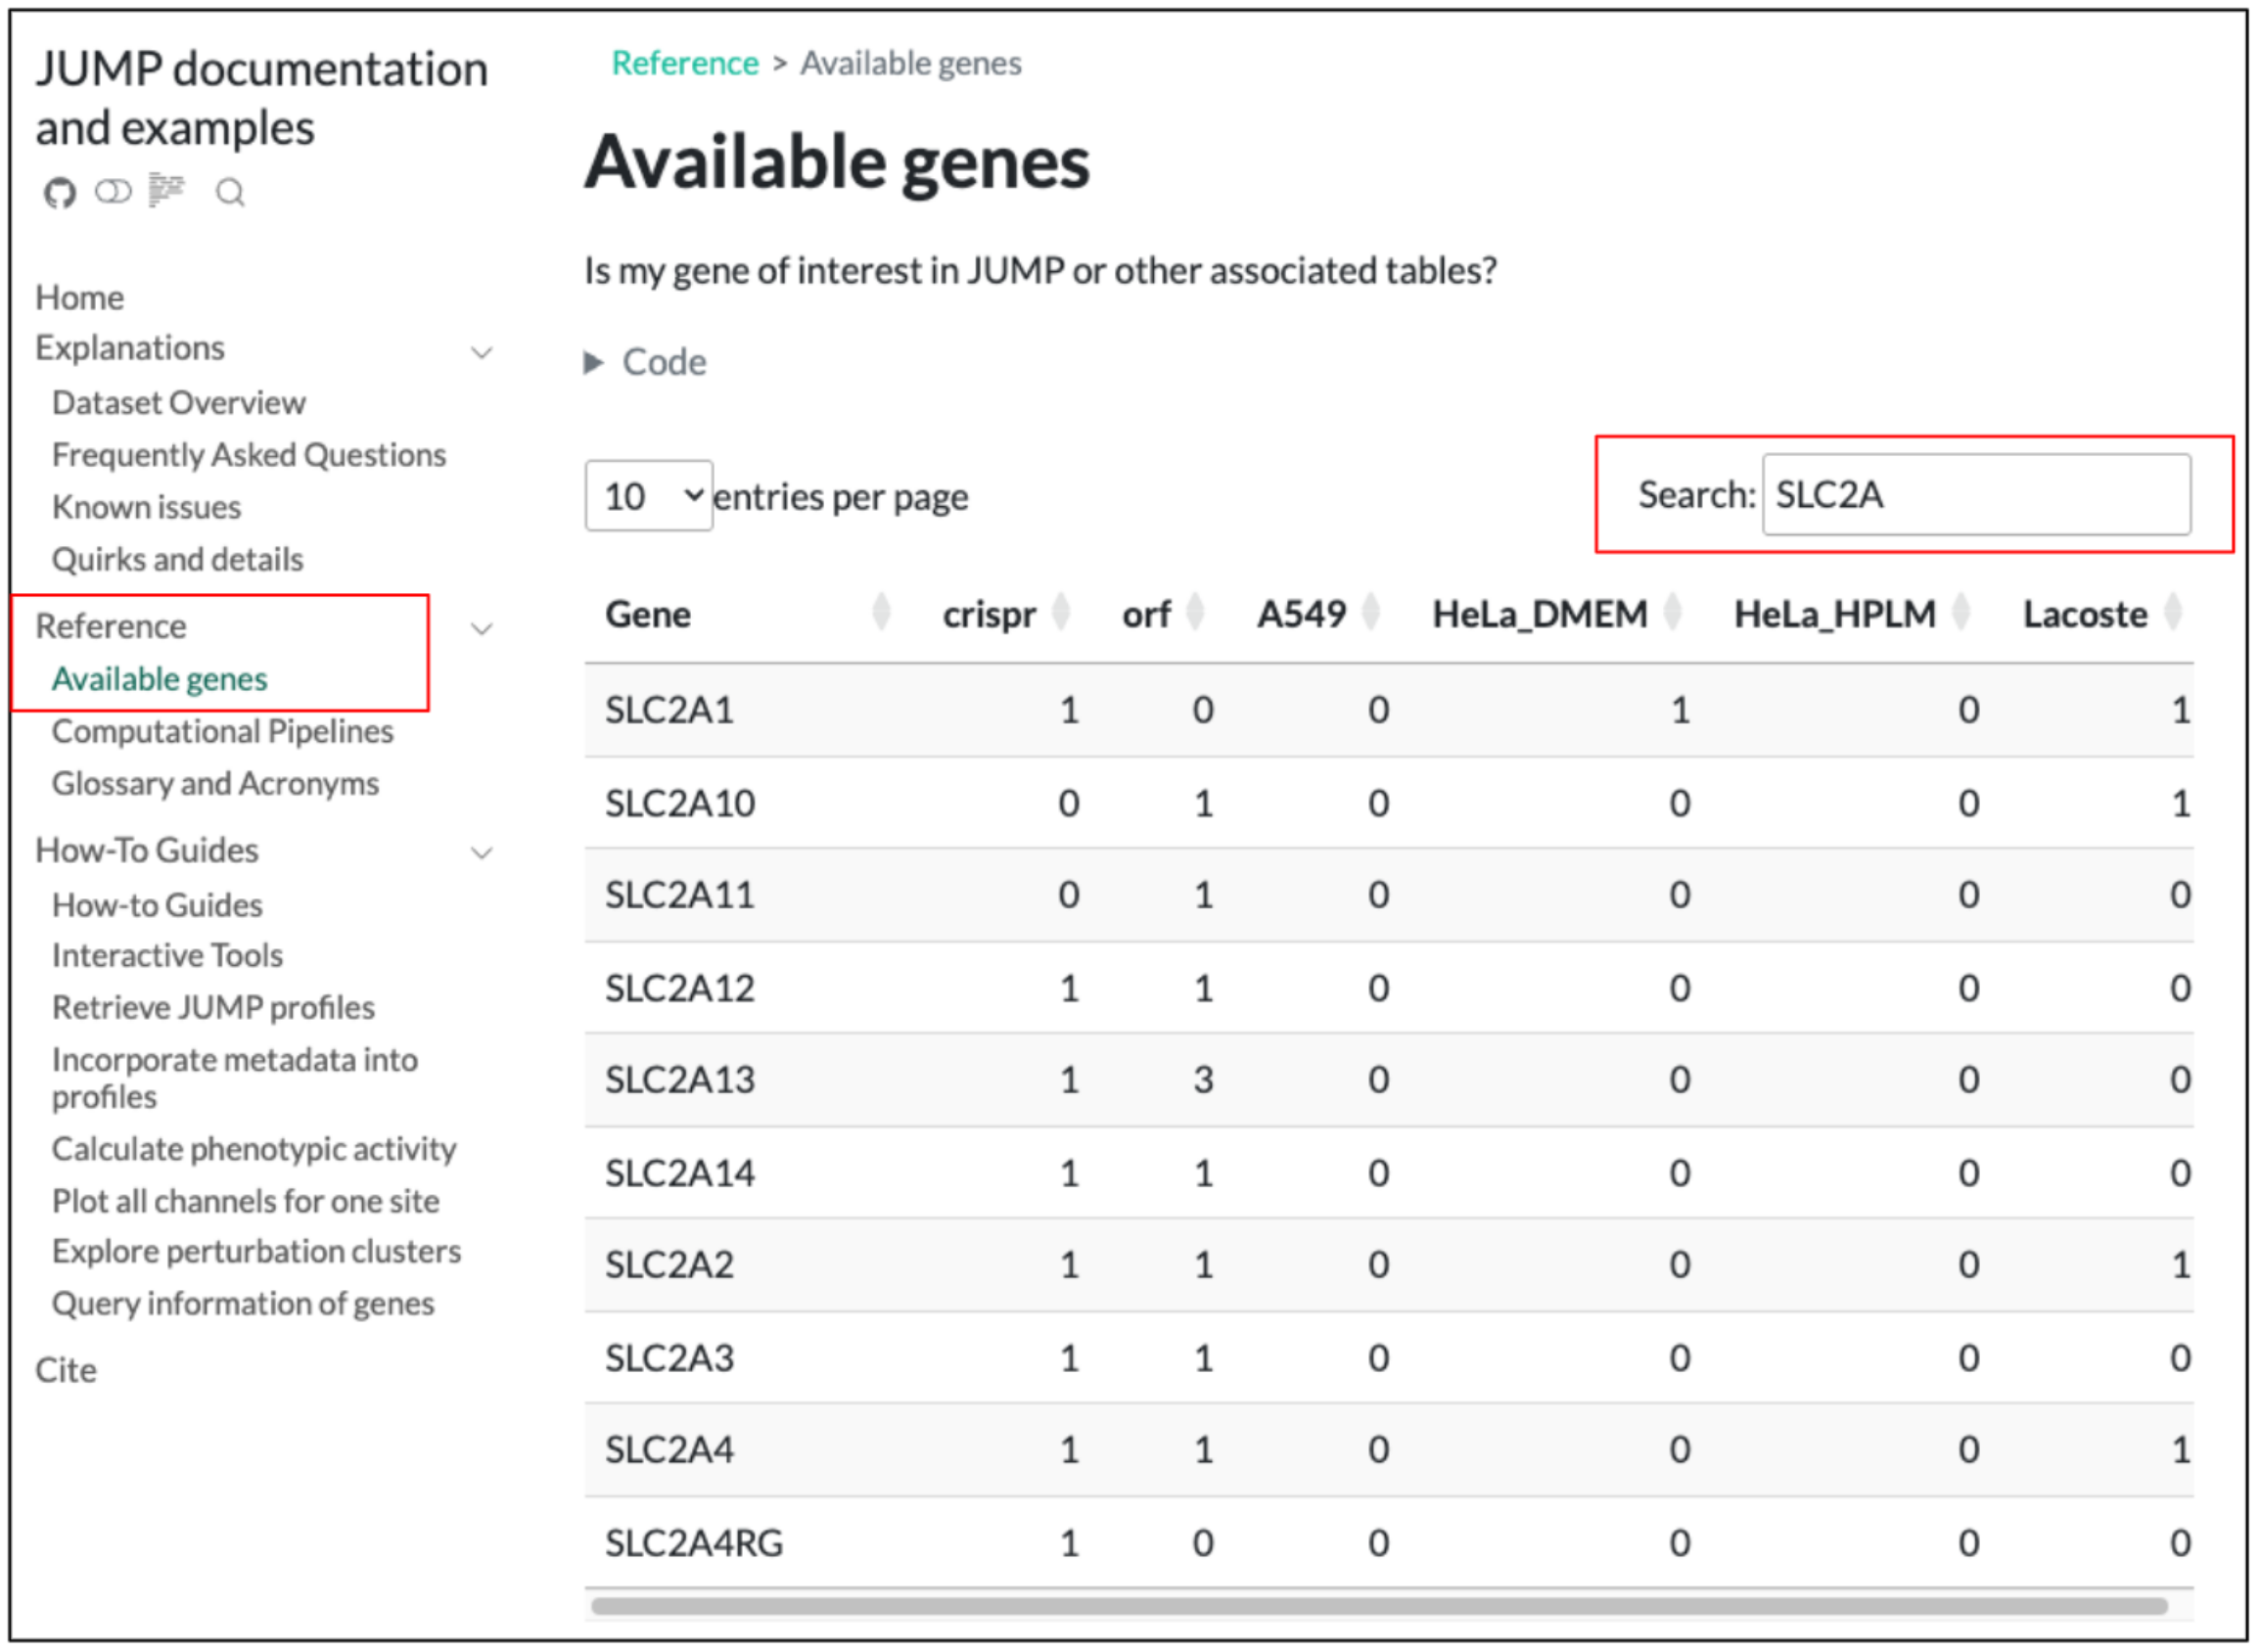
\includegraphics[width=0.98\linewidth,height=0.72\textheight,keepaspectratio]{assets/tutorial-screenshots/03-Figure3.png}
\par\medskip
{\footnotesize\raggedright\textbf{How:} search the availability table and read the CRISPR/ORF columns. Apply this to OPA1 and DNM1L.\par}
% Attribution: Broad Institute, JUMP Hub tutorial Fig. 3, https://zenodo.org/records/16878487, CC BY 4.0.
\end{frame}}

\newcommand{\TutorialDefinitionsSlide}{%
\begin{frame}[label={tutorial:interface}]{Which table columns answer our question?}
\centering
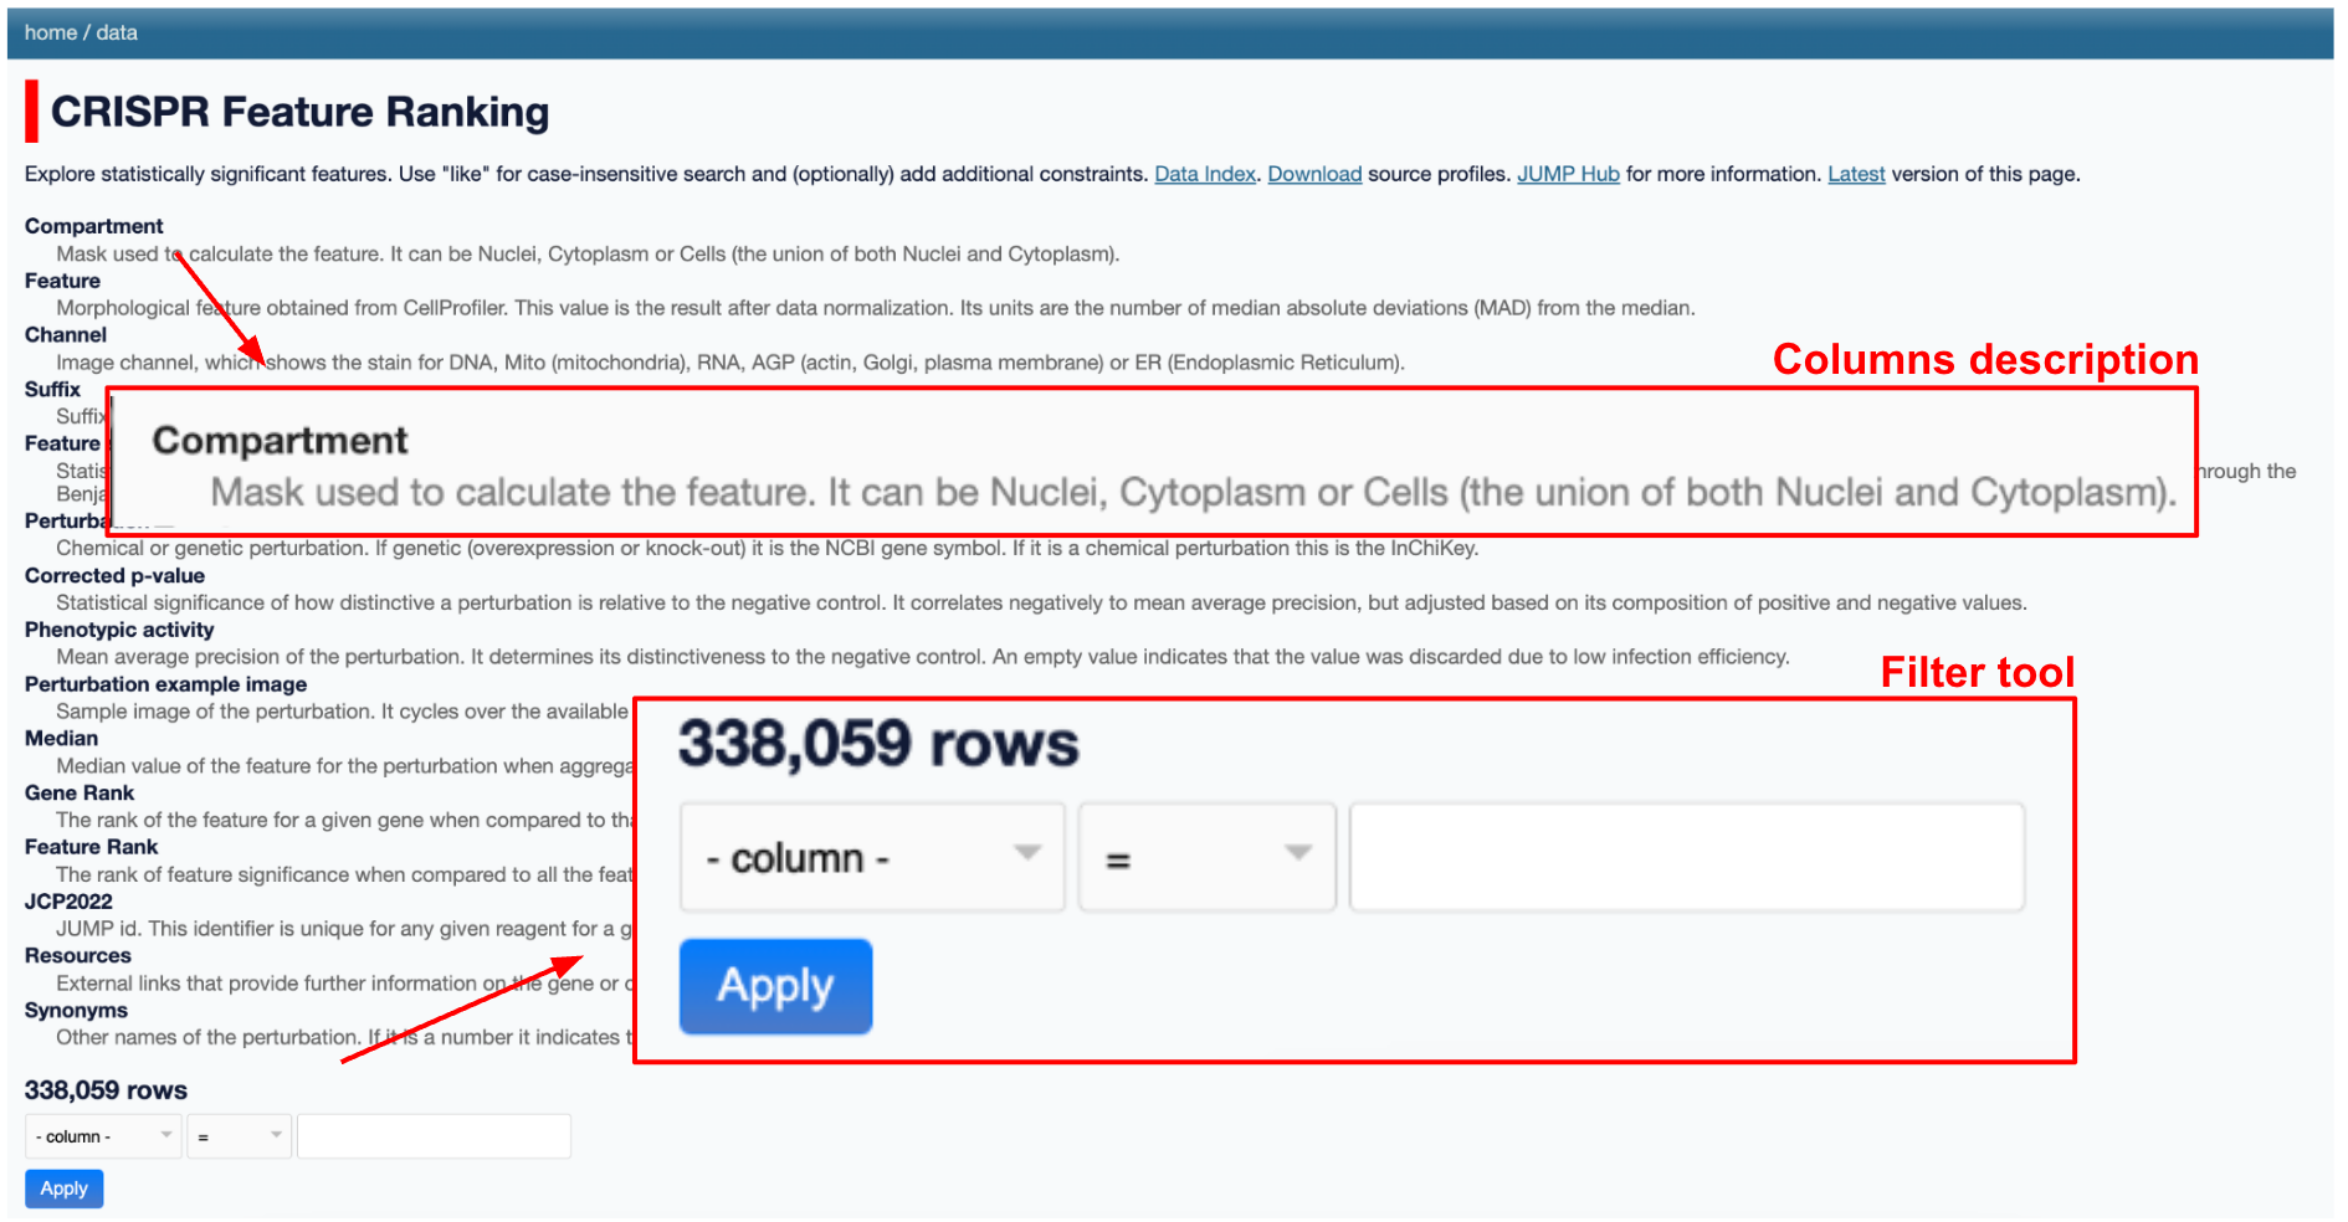
\includegraphics[width=0.98\linewidth,height=0.72\textheight,keepaspectratio]{assets/tutorial-screenshots/01-Figure1.png}
\par\medskip
{\footnotesize\raggedright\textbf{How:} use the column definitions to identify the gene, reagent, compartment, channel and result fields.\par}
% Attribution: Broad Institute, JUMP Hub tutorial Fig. 1, https://zenodo.org/records/15252378, CC BY 4.0.
\end{frame}}

\newcommand{\TutorialRowsSlide}{%
\begin{frame}[label={tutorial:rows}]{What does one feature result describe?}
\centering
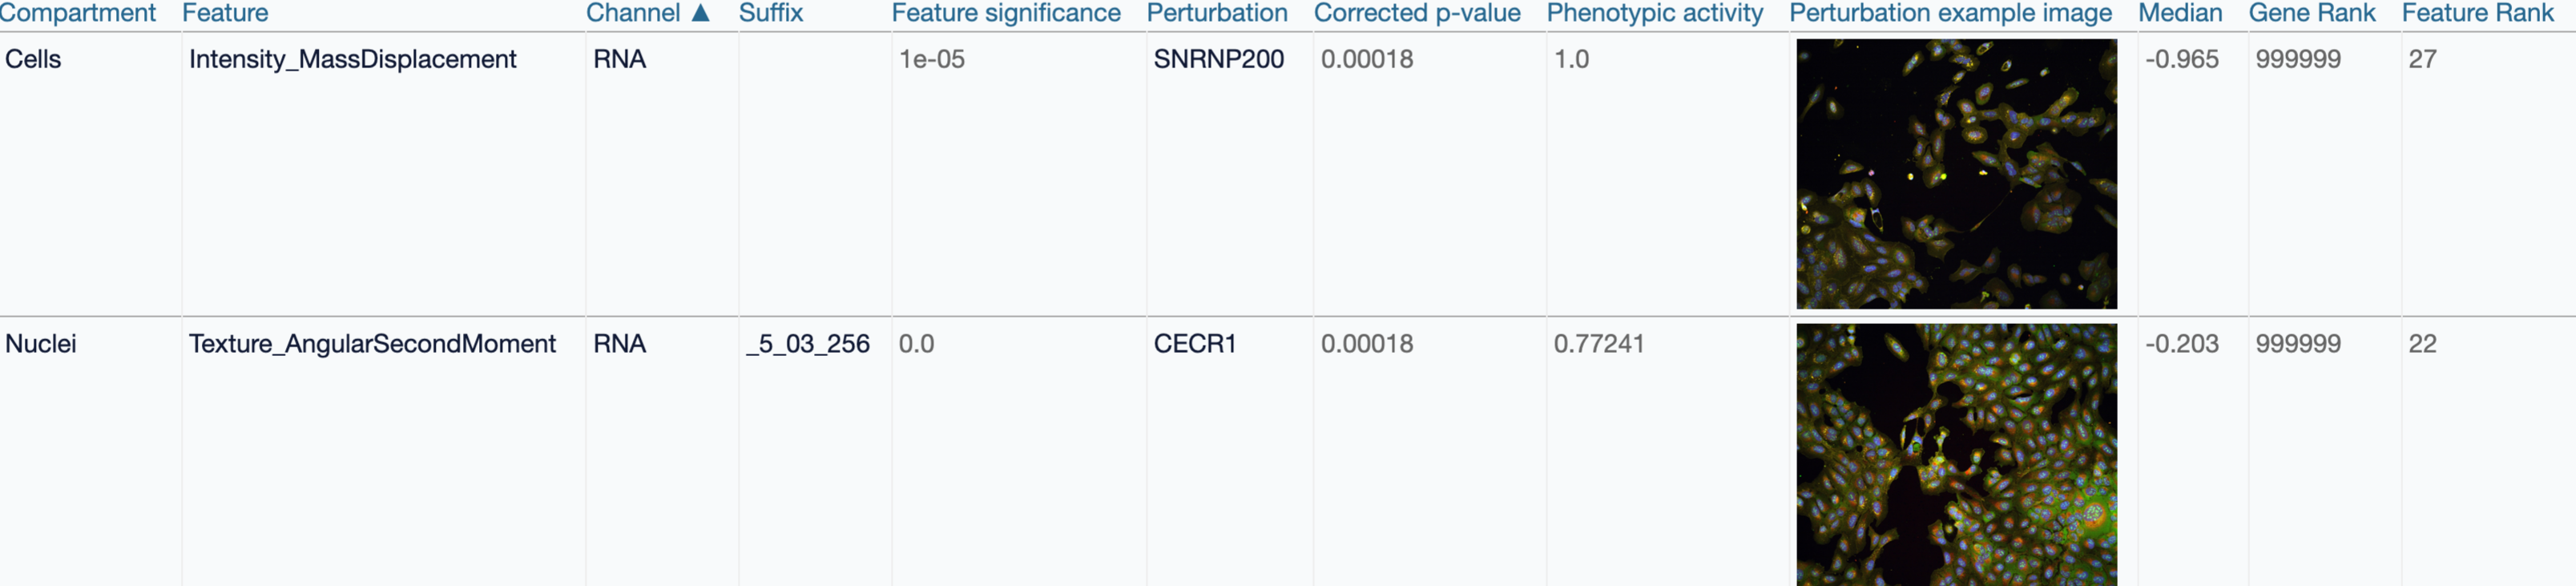
\includegraphics[width=0.98\linewidth,height=0.72\textheight,keepaspectratio]{assets/tutorial-screenshots/02-Figure2.png}
\par\medskip
{\footnotesize\raggedright\textbf{How:} read across a row: gene/reagent, measured feature, compartment, channel and statistical summary.\par}
% Attribution: Broad Institute, JUMP Hub tutorial Fig. 2, https://zenodo.org/records/15252378, CC BY 4.0.
\end{frame}}

\newcommand{\TutorialFiltersSlide}{%
\begin{frame}[label={tutorial:filters}]{How do we isolate the gene we care about?}
\centering
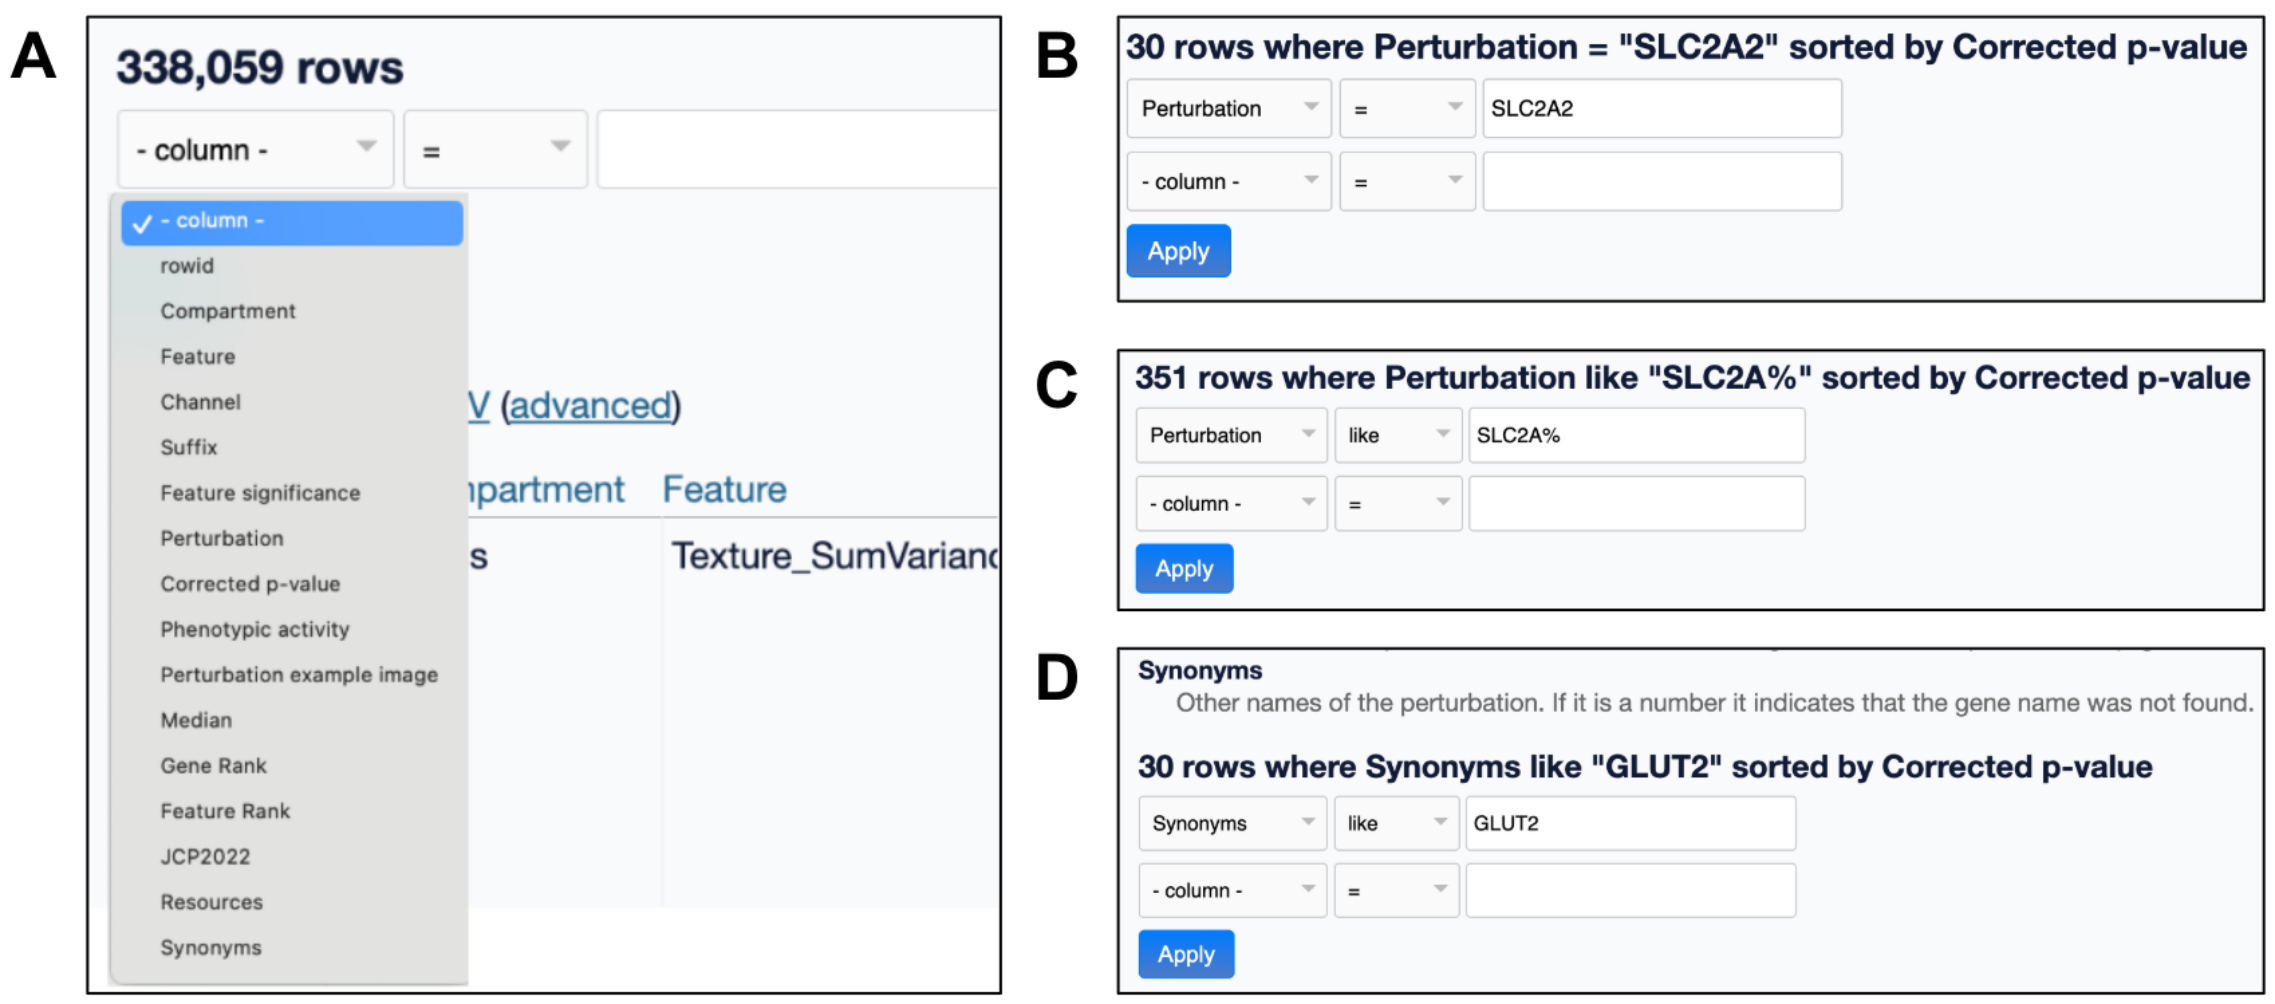
\includegraphics[width=0.98\linewidth,height=0.72\textheight,keepaspectratio]{assets/tutorial-screenshots/06-Figure4.png}
\par\medskip
{\footnotesize\raggedright\textbf{How:} filter by exact gene, family or synonym. Tutorial: SLC2A2 / SLC2A / GLUT2; use OPA1 or DNM1L for our examples.\par}
% Attribution: Broad Institute, JUMP Hub tutorial Fig. 4, https://zenodo.org/records/15252378, CC BY 4.0.
\end{frame}}

\newcommand{\TutorialExportSlide}{%
\begin{frame}[label={tutorial:export}]{How do we keep and share the result?}
\centering
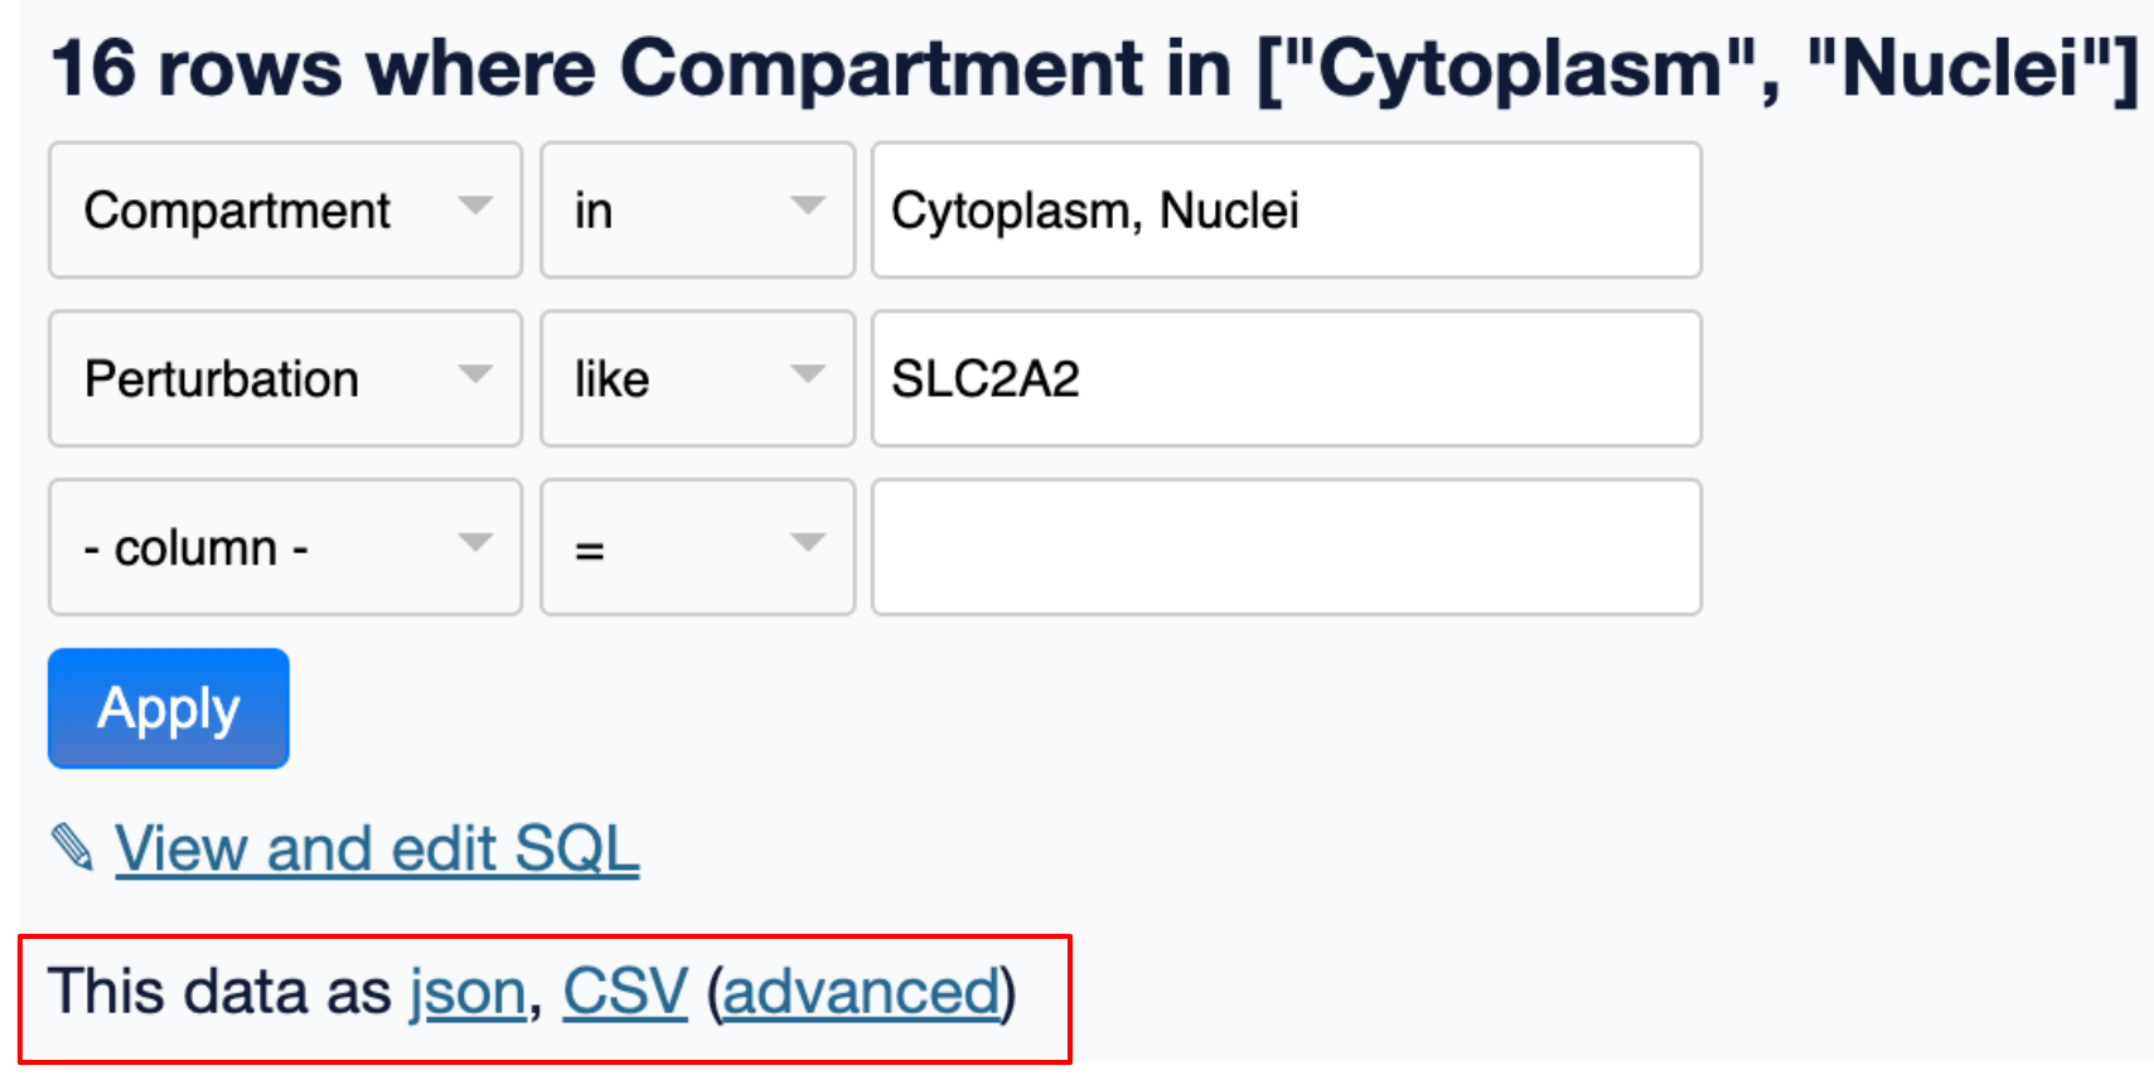
\includegraphics[width=0.98\linewidth,height=0.72\textheight,keepaspectratio]{assets/tutorial-screenshots/07-Figure5.png}
\par\medskip
{\footnotesize\raggedright\textbf{How:} keep the relevant compartments and export the filtered view with its gene, reagent and source link.\par}
% Attribution: Broad Institute, JUMP Hub tutorial Fig. 5, https://zenodo.org/records/15252378, CC BY 4.0.
\end{frame}}

\newcommand{\TutorialActivitySlide}{%
\begin{frame}[label={tutorial:activity}]{Does the perturbation have a measurable phenotype?}
\centering
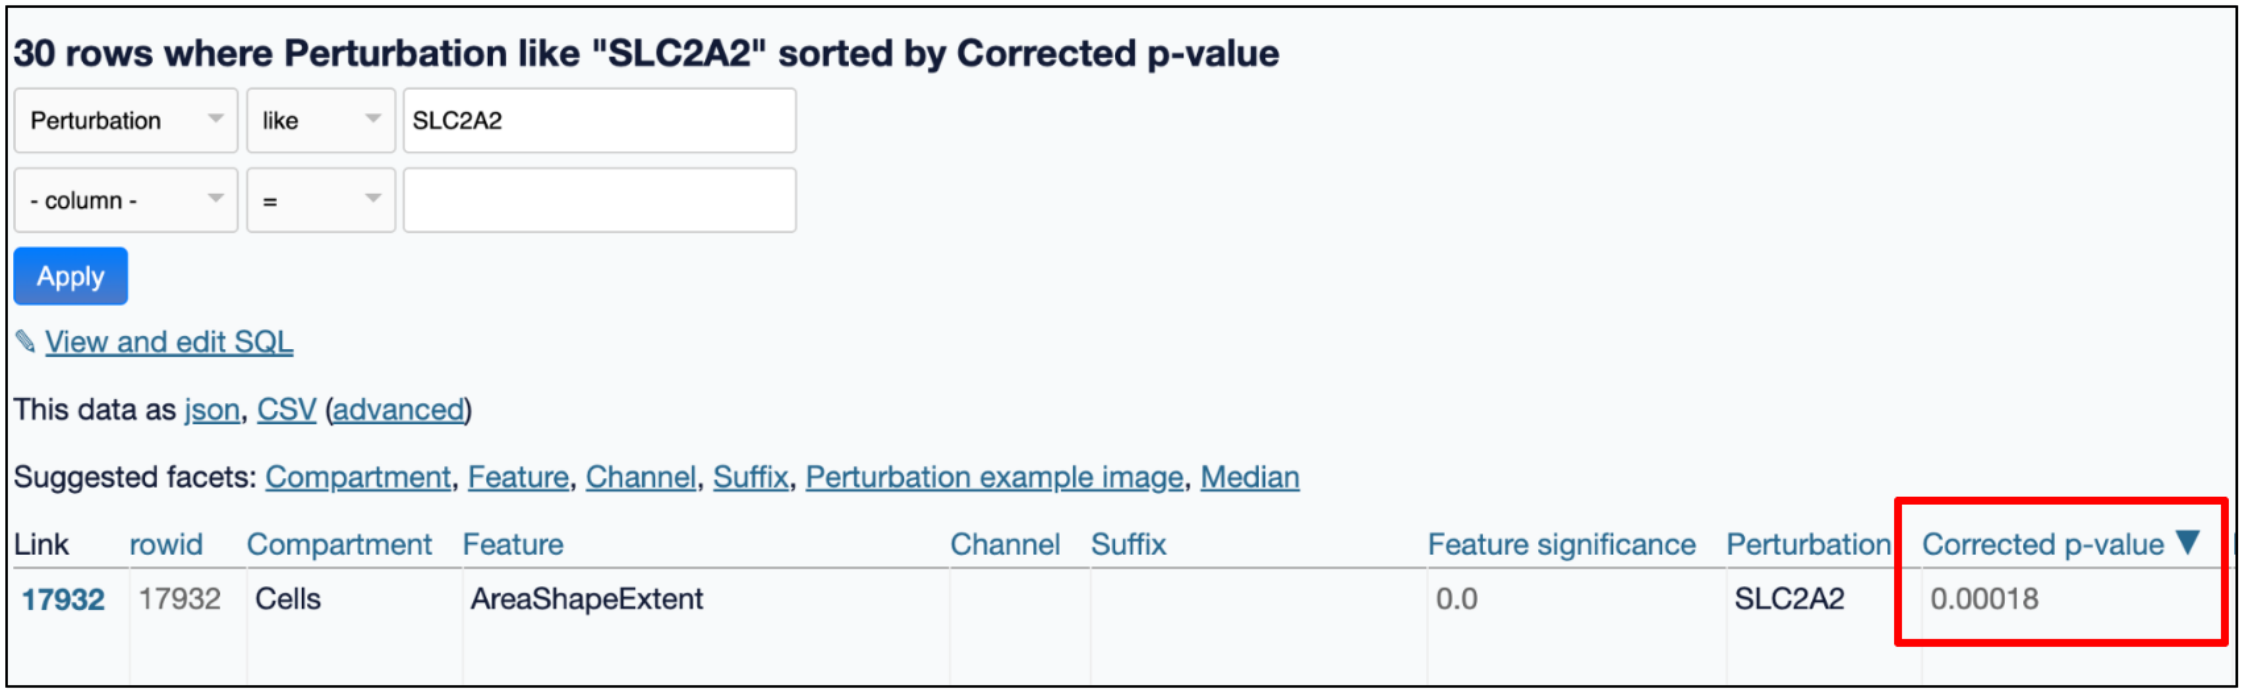
\includegraphics[width=0.98\linewidth,height=0.72\textheight,keepaspectratio]{assets/tutorial-screenshots/08-Figure6.png}
\par\medskip
{\footnotesize\raggedright\textbf{How:} select the gene in the CRISPR table; read phenotypic activity and the corrected p-value. Tutorial: SLC2A2.\par}
% Attribution: Broad Institute, JUMP Hub tutorial Fig. 6, https://zenodo.org/records/15252378, CC BY 4.0.
\end{frame}}

\newcommand{\TutorialFeaturesSlide}{%
\begin{frame}[label={tutorial:features}]{Which features explain the differences?}
\centering
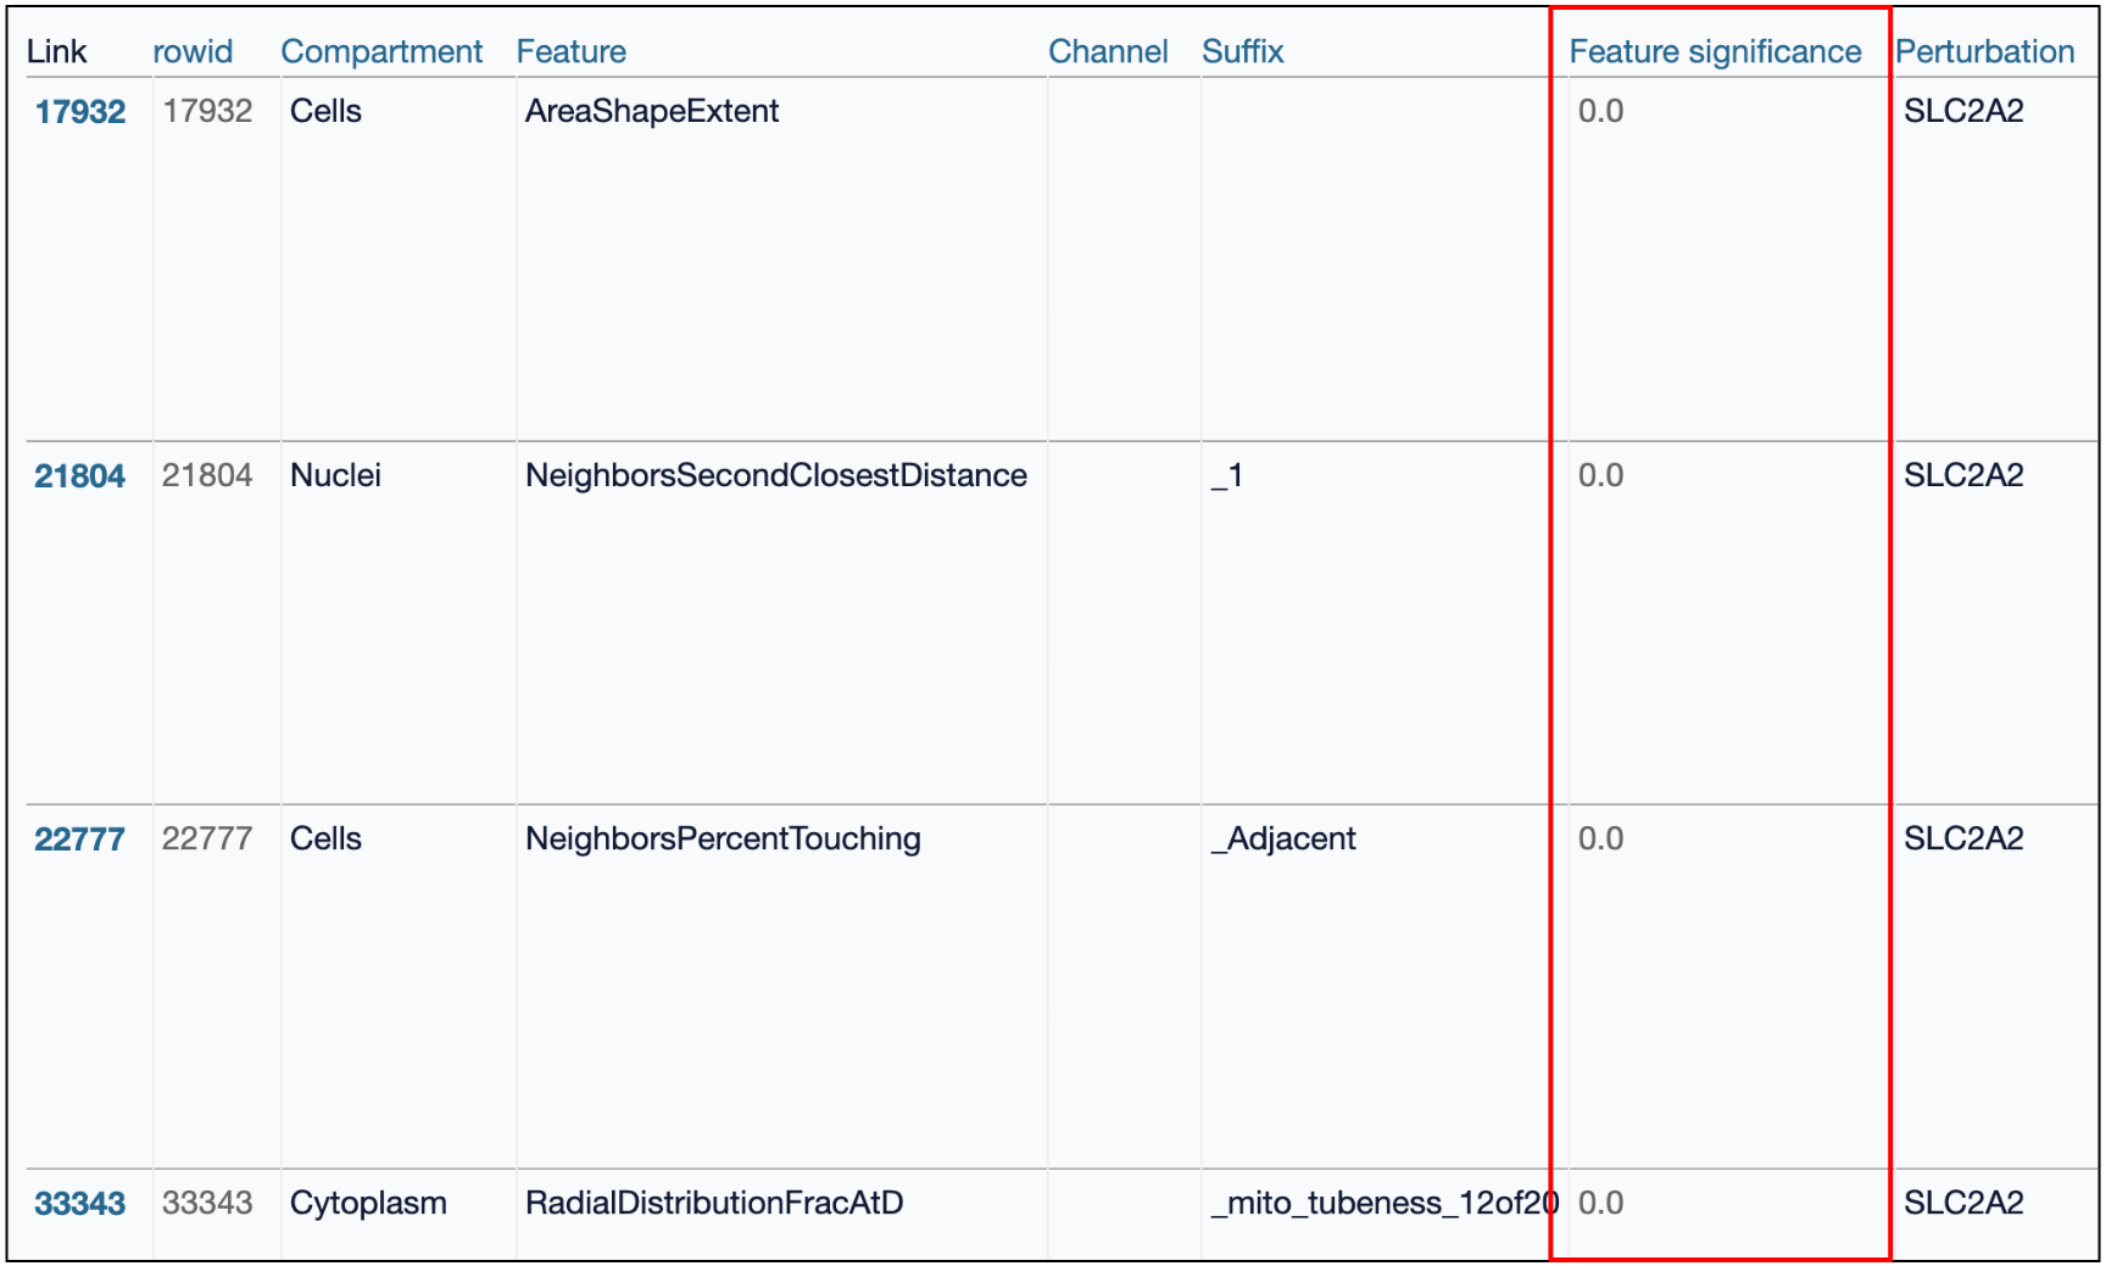
\includegraphics[width=0.98\linewidth,height=0.72\textheight,keepaspectratio]{assets/tutorial-screenshots/09-Figure7.png}
\par\medskip
{\footnotesize\raggedright\textbf{How:} inspect feature significance, rank and effect size; identify the relevant channels. Tutorial: SLC2A2; next: OPA1/DNM1L.\par}
% Attribution: Broad Institute, JUMP Hub tutorial Fig. 7, https://zenodo.org/records/15252378, CC BY 4.0.
\end{frame}}

\newcommand{\TutorialOrfSlide}{%
\begin{frame}[label={tutorial:orf}]{What happens with a different perturbation type?}
\centering
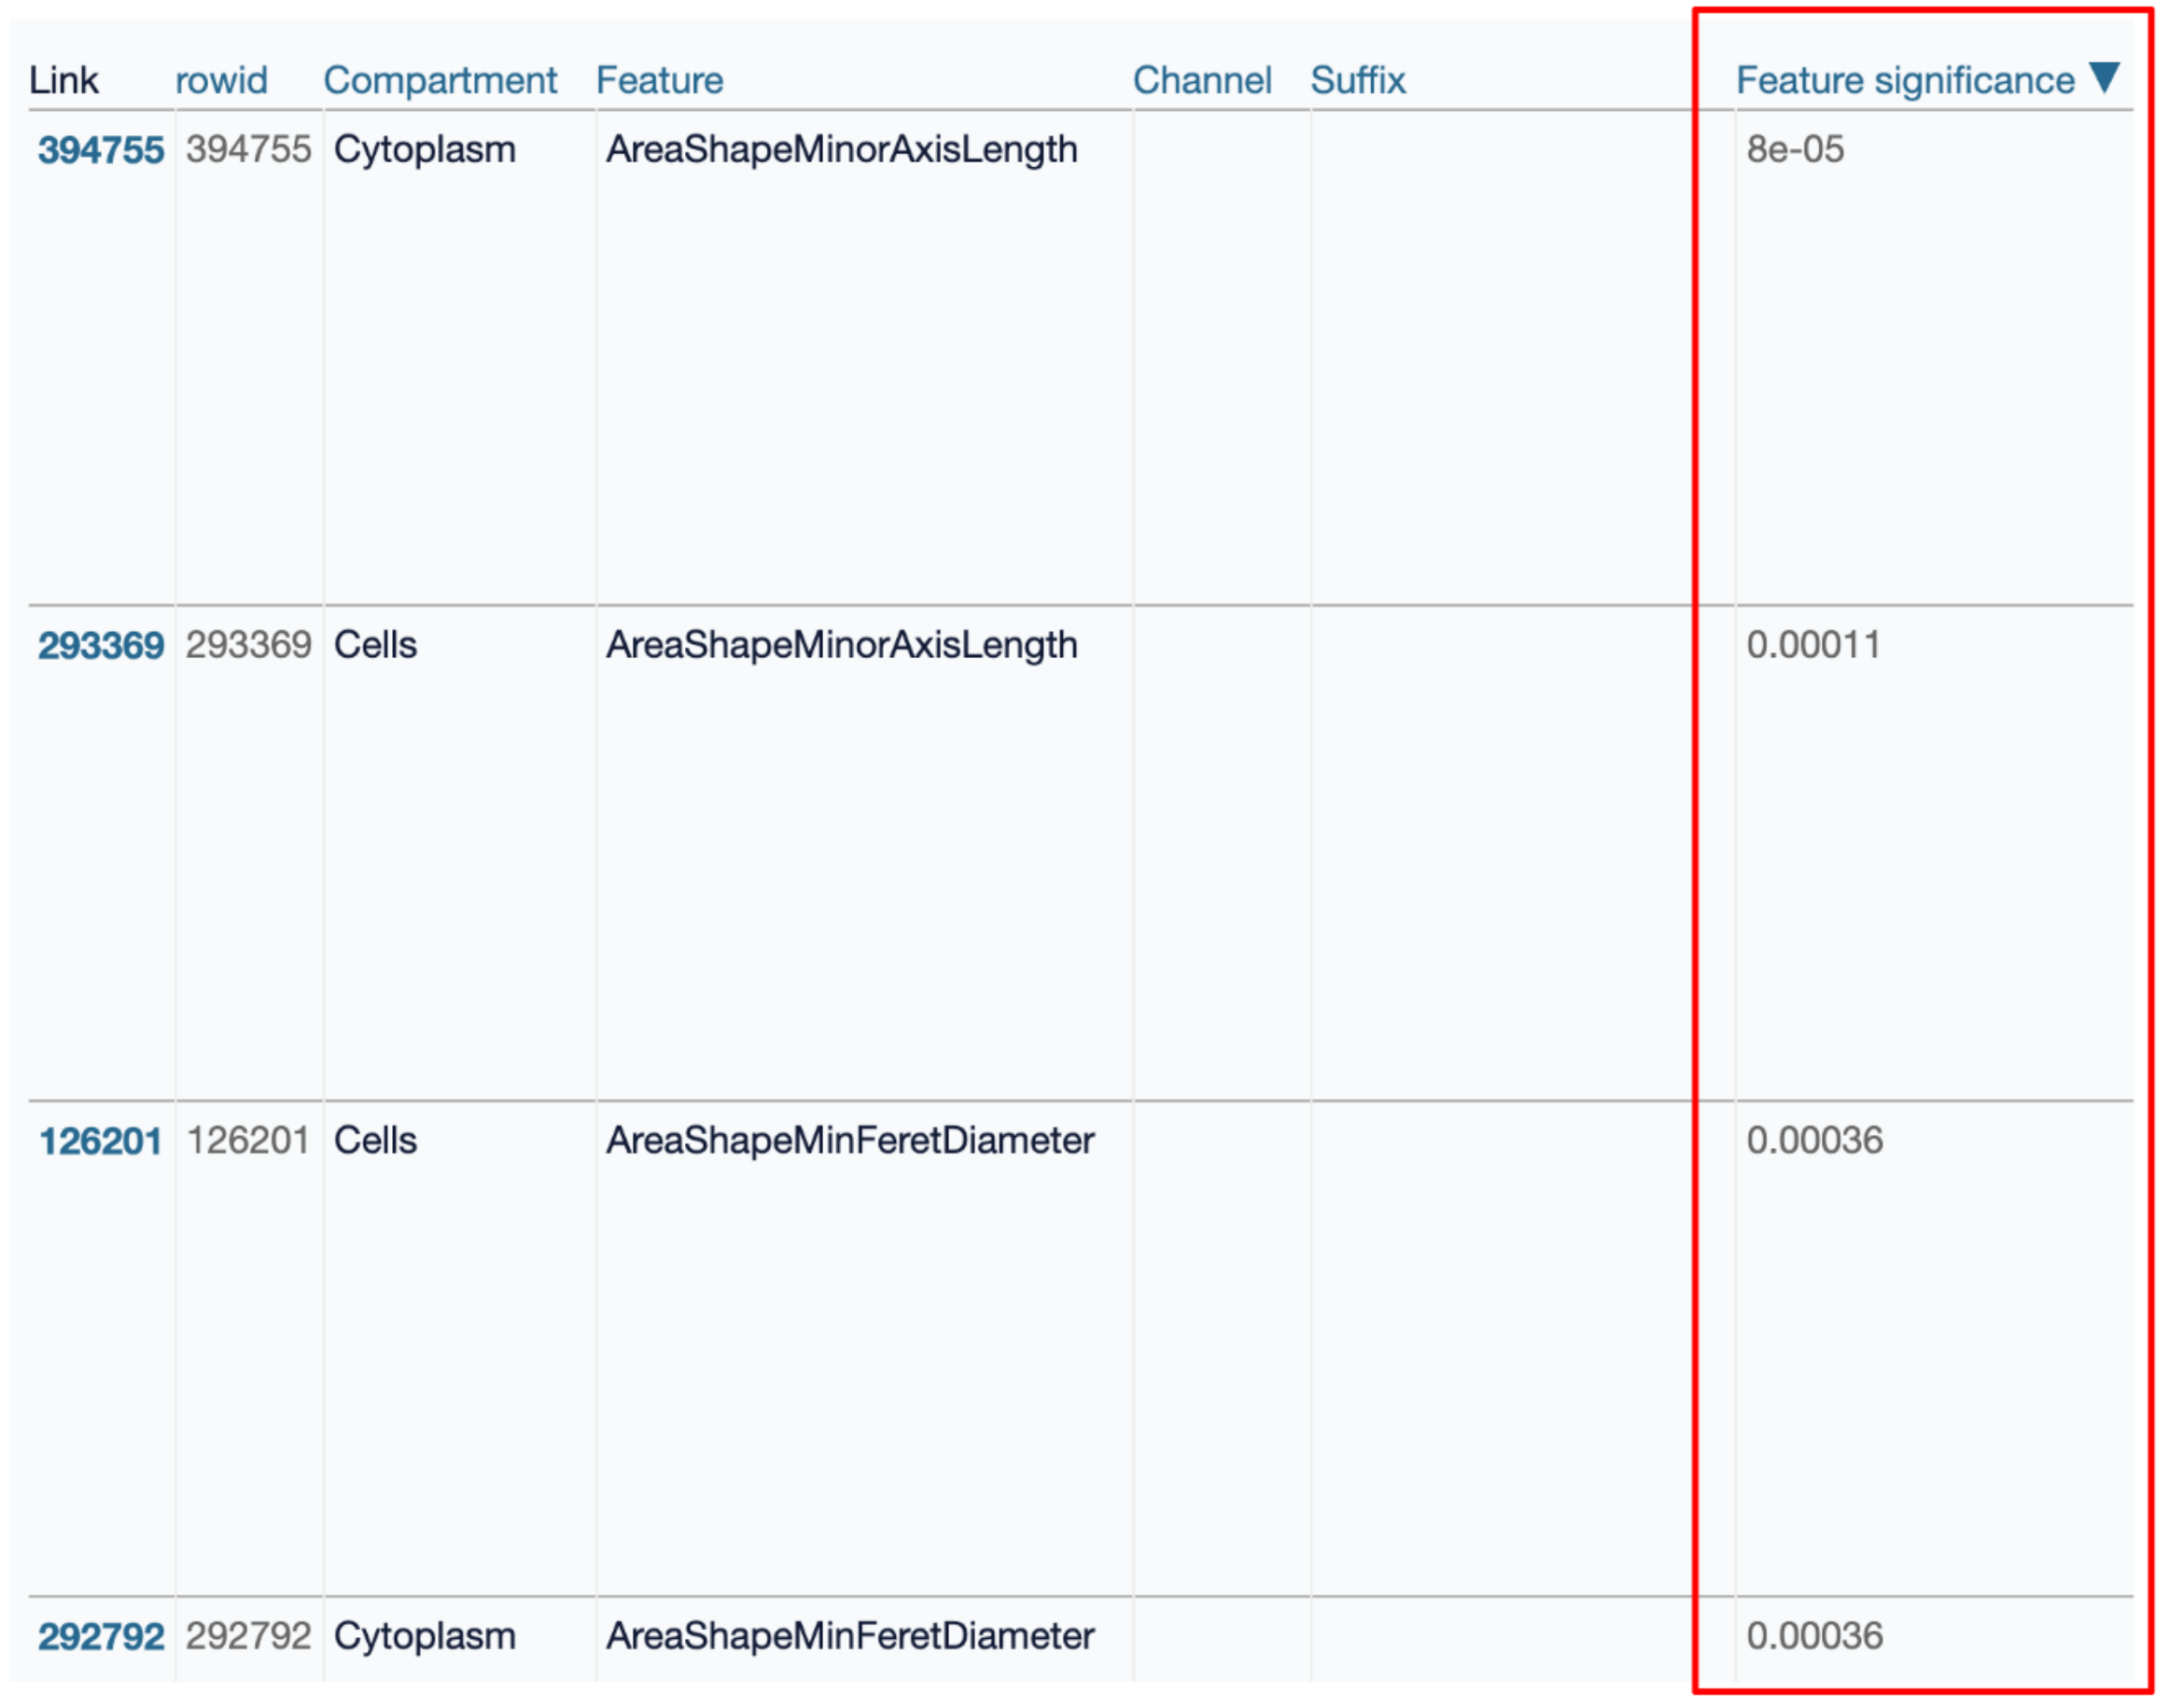
\includegraphics[width=0.98\linewidth,height=0.72\textheight,keepaspectratio]{assets/tutorial-screenshots/10-Figure8.png}
\par\medskip
{\footnotesize\raggedright\textbf{How:} open the ORF table for the same gene and compare activity and feature effects with CRISPR. Tutorial: SLC2A2.\par}
% Attribution: Broad Institute, JUMP Hub tutorial Fig. 8, https://zenodo.org/records/15252378, CC BY 4.0.
\end{frame}}

\newcommand{\TutorialMatchesSlide}{%
\begin{frame}[label={tutorial:matches}]{Which other perturbations have similar profiles?}
\centering
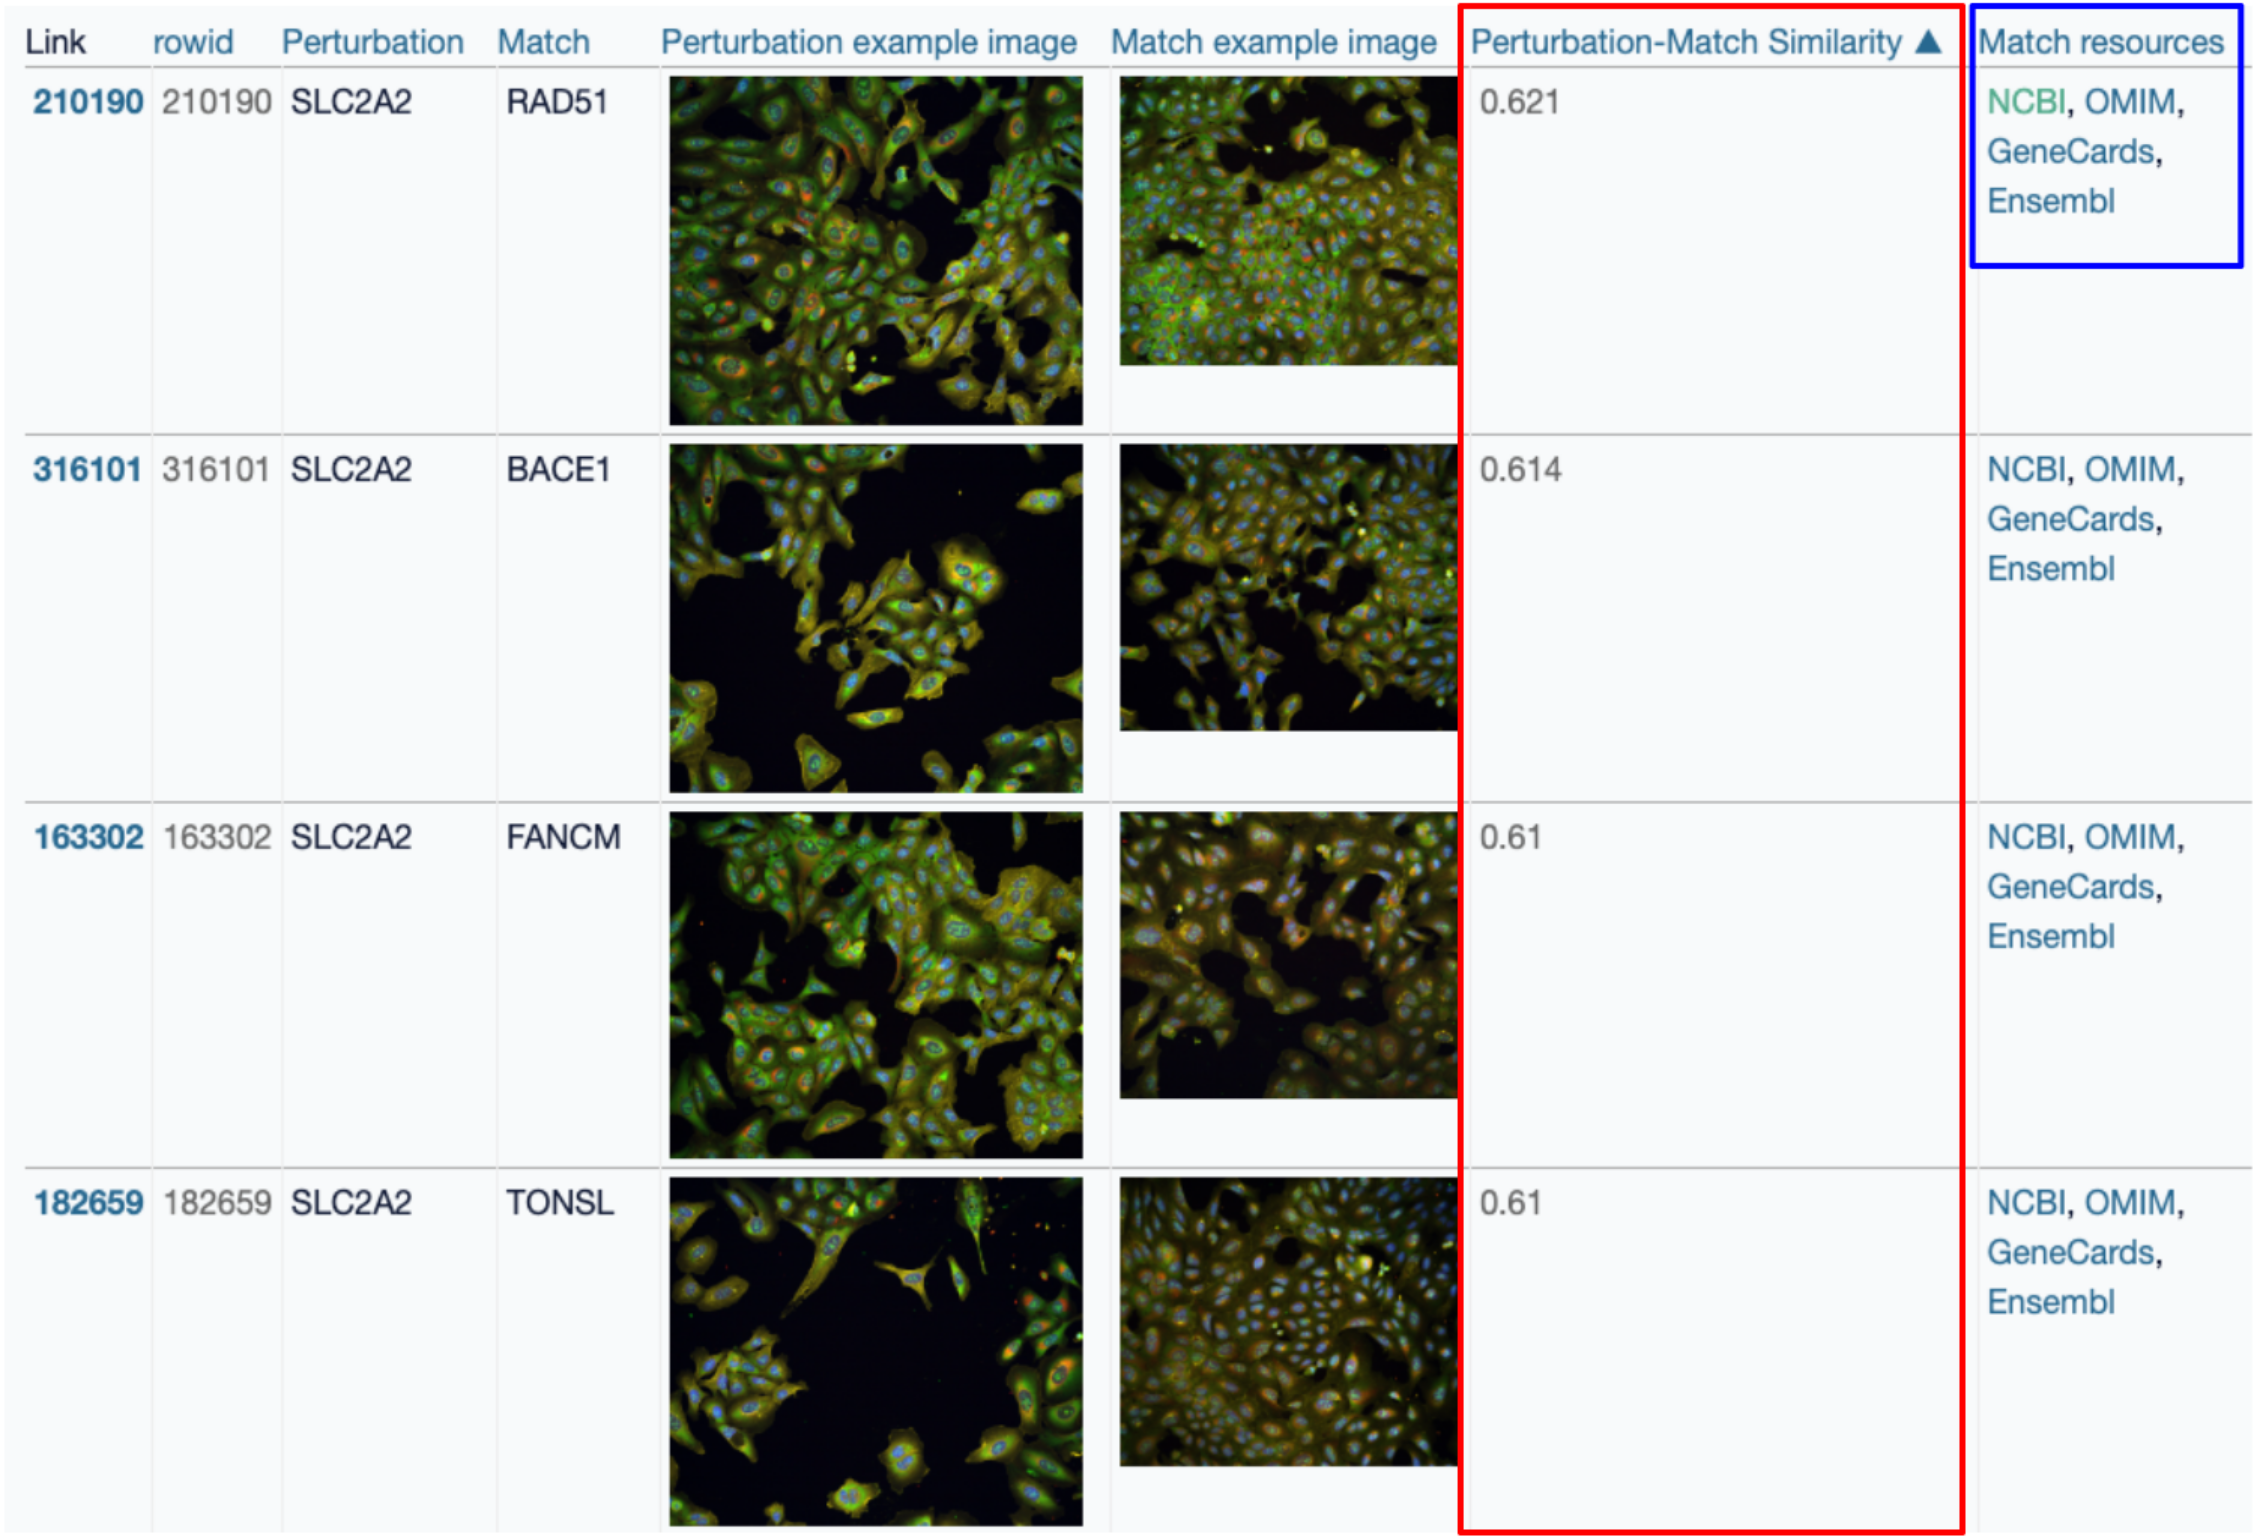
\includegraphics[width=0.98\linewidth,height=0.72\textheight,keepaspectratio]{assets/tutorial-screenshots/11-Figure9.png}
\par\medskip
{\footnotesize\raggedright\textbf{How:} filter the match table by gene, sort by signed similarity, and follow annotations and images. Tutorial: SLC2A2.\par}
% Attribution: Broad Institute, JUMP Hub tutorial Fig. 9, https://zenodo.org/records/15252378, CC BY 4.0.
\end{frame}}

\newcommand{\TutorialGallerySlide}{%
\begin{frame}[label={tutorial:gallery-perturbation}]{Where can we see the perturbed cells?}
\centering
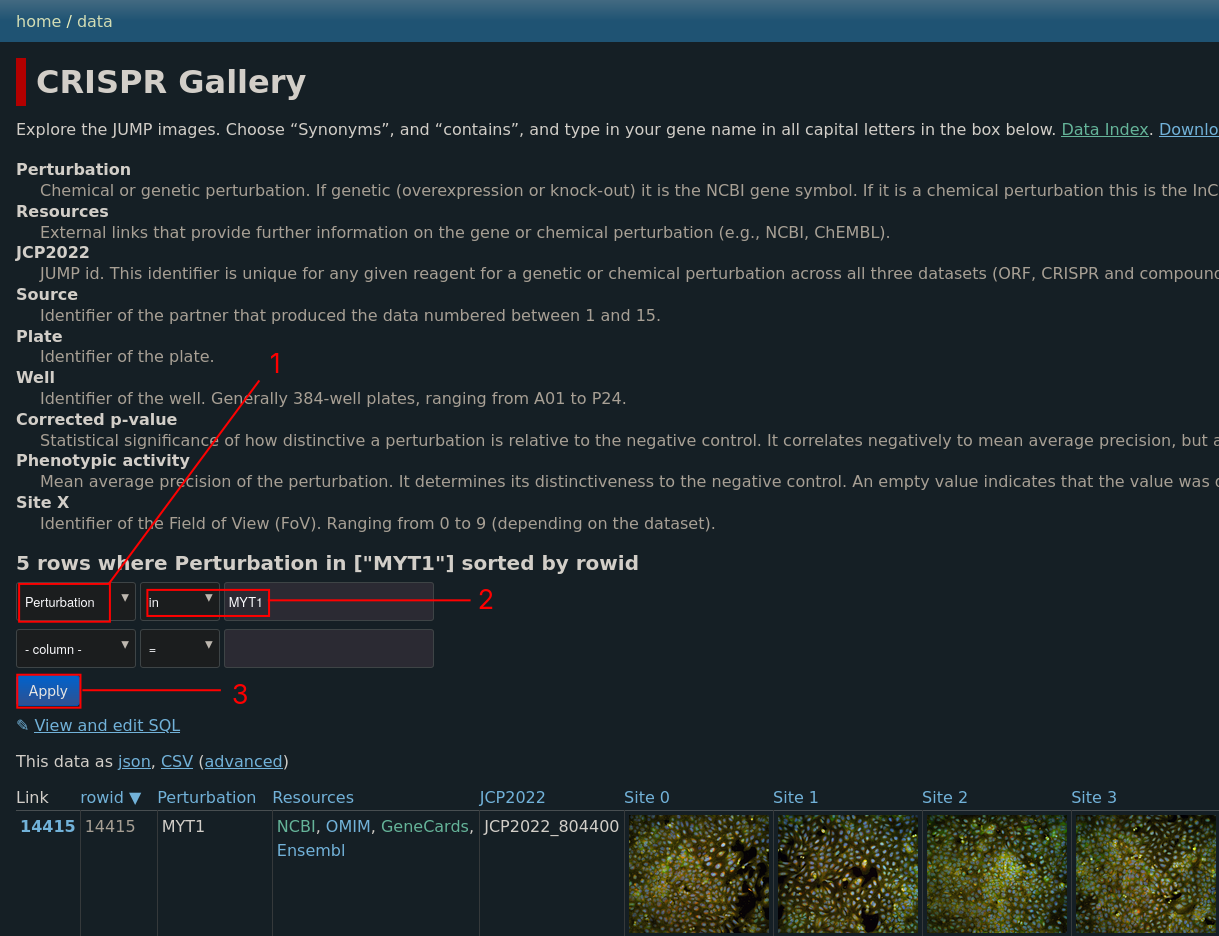
\includegraphics[width=0.98\linewidth,height=0.72\textheight,keepaspectratio]{assets/tutorial-screenshots/04-gallery_negcon_123.png}
\par\medskip
{\footnotesize\raggedright\textbf{How:} in the image table, filter by perturbation and identify the source and plates (steps 1--3). Tutorial: MYT1.\par}
% Attribution: Broad Institute, gallery tutorial steps 1--3, https://zenodo.org/records/16878778, CC BY 4.0.
\end{frame}}

\newcommand{\TutorialControlsSlide}{%
\begin{frame}[label={tutorial:gallery-controls}]{What should we compare those cells against?}
\centering
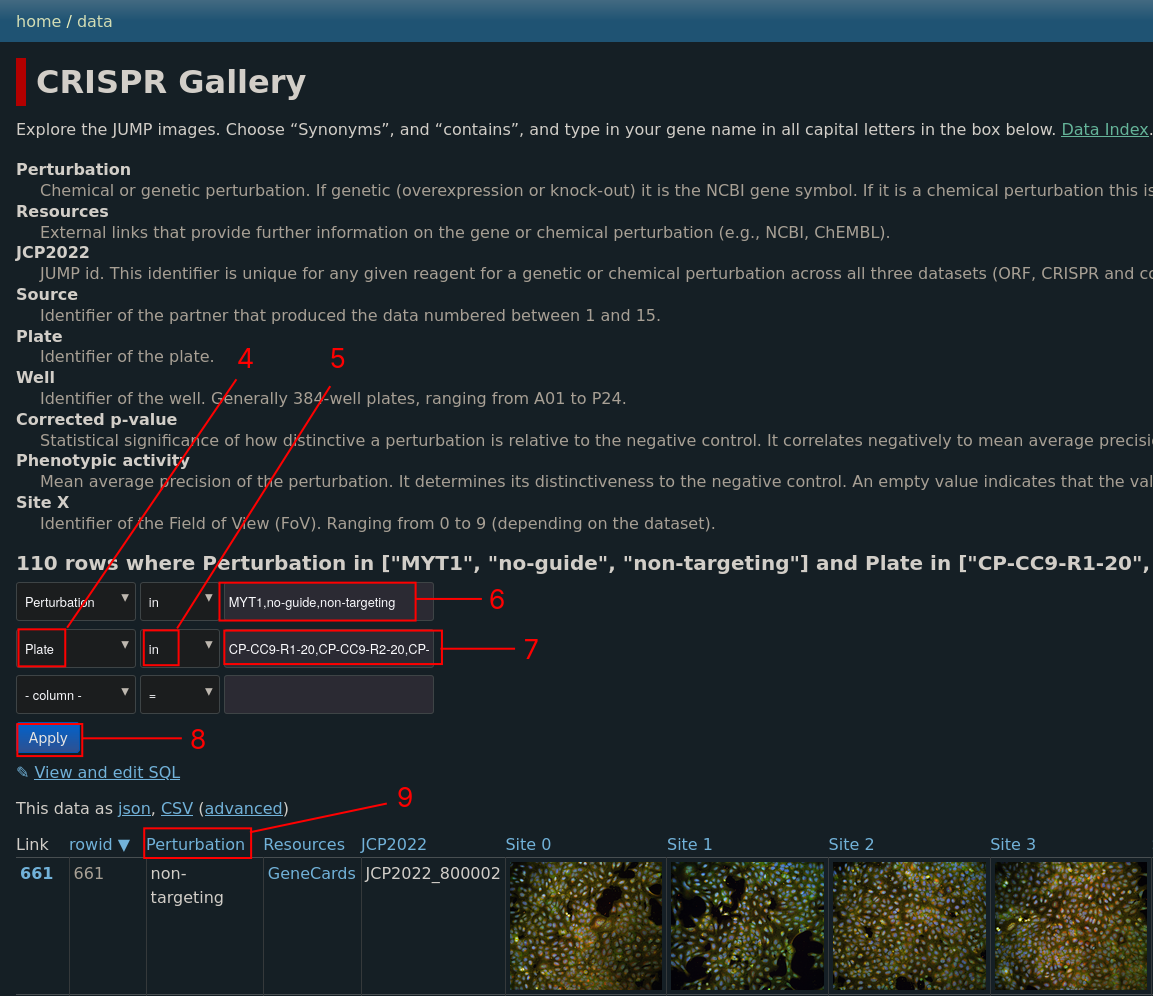
\includegraphics[width=0.98\linewidth,height=0.72\textheight,keepaspectratio]{assets/tutorial-screenshots/05-gallery_negcon_456789.png}
\par\medskip
{\footnotesize\raggedright\textbf{How:} retain the same source and plates, then include genetic negative controls (steps 4--9). Tutorial: MYT1.\par}
% Attribution: Broad Institute, gallery tutorial steps 4--9, https://zenodo.org/records/16878778, CC BY 4.0.
\end{frame}}
